\chapter{Volume flow boundary condition}

\modinfo{Directory}{FlowLinearRestriction}
\modinfo{Solvers}{\Idx{FlowSolve}, \Idx{SolveWithLinearRestriction}} 
\modinfo{Tools}{Editor, \Idx{Fortran 90 compiler}, \Idx{ElmerGrid}}
\modinfo{Dimensions}{2D, Transient}

\subsection*{Case definition}

This tutorial gives an example how to use SolveWithLinearRestriction. It also describes
how to execute own functions before the original system is solved. In order to
understand the case reader should be familiar with \Idx{compressed row storage} matrices and
Elmer basics. This tutorial gives only the guidelines and reader is advised to
read the files in order to get more through understanding.

We simulate the flow of incompressible fluid in a pipe.
The pipe has a length of 5 and a width of 1. On the left end we want to describe
a certain time dependent volume flow. In other words, we don't want to describe the velocity field
here but we want the velocity field be such that it transports certain amount of volume
in time interval. We could integrate the correct volume flow, but let's now approximate it
to make the more important aspects more visible. Our approximation here is that the volume
flow is proportional to average velocity on the edge i.e.
\begin{equation}
\frac{1}{N}\sum_{i=1}^{N}u_i = \frac{volume}{time}
\end{equation}
Here $u_i$ are the nodal velocities parallel to the pipe on the left edge and $N$ is the number of nodes on
the left edge. We want to set a nicely scaled sinusoidal volume flow on the edge, which leads to
\begin{equation}
\sum_{i=1}^{N}u_i = 10N\sin(2\Pi t)
\end{equation}
This equation we can (easily) force with Lagrange multiplier.

\subsection*{Solution procedure}
First we make a uniform mesh of 800 four-node quadrilaterals with command
\ttbegin
ElmerGrid 1 2 mflow
\ttend
Next we construct the solver input file. Header is simply
\ttbegin
Header
  Mesh DB "." "mflow"
End
\ttend
The simulation block is also very simple. 
Here we need to define the time stepping method and timescale.
\ttbegin
Simulation
  Coordinate System = Cartesian 2D

  Simulation Type = Transient
  Steady State Max Iterations = 1

  Timestepping Method = BDF
  BDF Order = 1

  Timestep Sizes = 0.02
  Timestep Intervals = 100

  Output Intervals = 1

  Output File = "mflow.result"
  Post File = "mflow.ep"
End
\ttend
The body, material and equation blocks are as usual. The material parameters,
of course, have affect on the solution and interested reader is encouraged to
modify these values and recalculate the solution.
\ttbegin
Body 1
  Material = 1
  Equation = 1
End

Material 1
  Density = 3.0
  Viscosity = 0.1
End

Equation 1
  Navier-Stokes = TRUE
  Active Solvers(1) = 1
End
\ttend
The solver block has the usual Navier-Stokes keywords and two keywords
for volume flow boundary. 
The {\tt Before Linsolve} keyword defines binary file and function that is
called before the system is solved. This function we must write and
compile and we will come to it shortly. The following keyword,
{\tt Export Lagrange Multiplier}, states that we are not interested in 
the value of the Lagrange multiplier and it is therefore not saved.
\ttbegin
Solver 1
  Equation = Navier-Stokes
  Stabilize = True

  Before Linsolve = "./AddMassFlow" "AddMassFlow"
  Export Lagrange Multiplier = Logical FALSE

  Linear System Solver = Iterative
  Linear System Iterative Method = BiCGStab
  Linear System Preconditioning = ILU1
  Linear System Max Iterations = 500
  Linear System Scaling = False
  Linear System Convergence Tolerance = 1.0e-8

  Nonlinear System Max Iterations = 15
  Nonlinear System Convergence Tolerance = 1.0e-8
  Nonlinear System Newton After Tolerance = 1.0e-4
  Nonlinear System Newton After Iterations = 8
  Nonlinear System Relaxation Factor = 1.0

  Steady State Convergence Tolerance = 1.0e-7
End
\ttend
In boundary conditions we state that both parallel and perpendicular velocities
are zero on the pipe sides and on both edges the perpendicular velocity is zero.
Here we also define the number tags for the boundaries. The tag 2 is assigned to
boundary that has number 4 in grd-file, which is the left edge of the pipe.
To this tag number 2 we shall refer in our AddMassFlow-function.
\ttbegin
Boundary Condition 1
  Target Boundaries(2) = 1 3
  Velocity 1 = 0.0
  Velocity 2 = 0.0
End

Boundary Condition 2
  Target Boundaries = 4
  Velocity 2 = 0.0
End

Boundary Condition 3
  Target Boundaries = 2
  Velocity 2 = 0.0
End
\ttend
\subsection*{AddMassFlow function}
Here we shall only give some rough guidelines of the function, for more information
check the code. This function creates the constraint matrix and RHS that forces the
equation mentioned above. Then it calls SolveWithLinearRestriction to solve the system.
The constraint matrix is actually only a row-vector and the RHS is only one value. 
\begin{itemize}
\item The function parameters are defined in Elmer so you shouldn't change them.
\item First we set a pointer to EMatrix-field of the given system matrix.
If the pointed matrix is not yet allocated, calculate the number of nodes
on the edge we want to define the volume flow. This gives us the number of non-zeros
in our constraint matrix and we can allocate the matrix.
\item Set the rows, cols and diag -fields of the matrix. This sets the non-zeros
on their right places in the constraint matrix.
\item Set all values of the constraint matrix to unity.
\item Calculate the RHS-value. The current time was checked in the beginning 
of the function, so this is possible.
\item Call SolveWithLinearRestriction
\item Return 1 which tells the ElmerSolver that the system is already solved.
\end{itemize} 
The function is the compiled with command
\ttbegin
elmerf90 -o AddMassFlow AddMassFlow.f90 
\ttend
Here it is assumed that the source file name is AddMassFlow.f90.

\subsection*{Results}
Just say {\tt ElmerSolver} and you should get the solution in few minutes.
The velocity perpendicular to the pipe is practically zero and the velocity
parallel to the pipe is an example of \Idx{Womersley velocity profile}
\footnote{J.Physiol (1955) 127, 553-563}.
An interesting feature of this velocity profile is that on some time steps 
the fluid flows to both directions, see figure~\ref{f:womersley}.
\begin{figure}[!hb]
\begin{center}
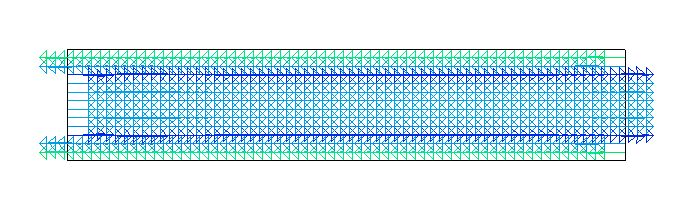
\includegraphics[width=\textwidth]{womersley}
\caption{Solution of the velocity field. Note the flow to both directions.}
\label{f:womersley}
\end{center}
\end{figure}

